\documentclass[12pt]{report}
  \usepackage[T1]{fontenc}
  \usepackage[french]{babel}
  \usepackage[utf8x]{inputenc}
  \usepackage{amsmath}
  \usepackage{graphicx}
  \usepackage{wrapfig}
  \usepackage{caption}
  \usepackage[colorinlistoftodos]{todonotes}
  \usepackage[strings]{underscore}
  \usepackage{url}
  \usepackage{hyperref}
  \usepackage{soul}
  
  \hypersetup{%
      pdfborder = {0 0 0}
  }
  
  \begin{document}
  
  
  \newcommand{\source}[1]{\caption*{Source: {#1}} }
  
  %-----------------------------------------------------------------%
  %    PAGE DE TITRE
  %-----------------------------------------------------------------%
  
  \begin{titlepage}
  
  \newcommand{\HRule}{\rule{\linewidth}{0.7mm}} % Trait horizontal
  
  \center
   
  %---------------------------%
  %   LOGO & EN-TÊTE DE PAGE
  %---------------------------%
  
\includegraphics[width=0.8\textwidth]{img/logo.jpg}\\
  
  \textsc{\Large Projet de Programmation}\\[0.5cm]
  \textsc{\large Génération procédurale de planètes}\\[0.5cm]
  
  %---------------------------%
  %   TITRE
  %---------------------------%
  
  \HRule \\[0.4cm]
  { \huge \bfseries Rapport}\\[0.4cm]
  \HRule \\[1.5cm]
   
  %---------------------------%
  %   AUTHEURS
  %---------------------------%
  
  \begin{minipage}{0.4\textwidth}
  \begin{flushleft} \large
  \emph{Auteurs:}\\
  Rémy \textsc{Maugey}\\
  Jérémi \textsc{Bernard}\\
  Hugo \textsc{Alonso}\\
  Brian \textsc{Mazé}\\
  \end{flushleft}
  \end{minipage}
  ~
  \begin{minipage}{0.4\textwidth}
  \begin{flushright} \large
  \emph{Client:} \\
  Emmanuel \textsc{Fleury}
  \end{flushright}
  ~
  \begin{flushright} \large
  \emph{Chargé de TD:} \\
  Boris \textsc{Mansencal}
  \end{flushright}
  \end{minipage}\\[2cm]
  
  %---------------------------%
  %   DATE
  %---------------------------%
  
  {\large 05 Avril 2018\\[2cm] }
  
  
  \vfill % Fill the rest of the page with whitespace
  
  \end{titlepage}
  %-----------------------------------------------------------------%
  %   FIN PAGE DE TITRE
  %-----------------------------------------------------------------%
  
  
  
  
  
  
  
  
  
  %-----------------------------------------------------------------%
  %   Table des Matières
  %-----------------------------------------------------------------%
  
  
  \tableofcontents
  
  \thispagestyle{empty} % empeche l'affichage du numero de cet page
  
  
  
  
  
  
  
  
  
  
  
  
  
  
  
  
  
  %-----------------------------------------------------------------%
  %   Introduction
  %-----------------------------------------------------------------%
  
  \newpage
  
  \chapter*{Introduction}
  \addcontentsline{toc}{chapter}{Introduction}
  \setcounter{chapter}{0}
  
  
  
  
  
  
  
  
  
  
  
  
  
  
  %-----------------------------------------------------------------%
  %   Algorithme CDLOD
  %-----------------------------------------------------------------%
  
  
  \newpage
  
  \chapter{Algorithme CDLOD}

  L'algortihme \textbf{CDLOD}, pour "Continuous Distance-Dependent Level of Detail for Rendering Heightmaps " 
  (Niveau de détail continu dépendant de la distance pour le rendue de carte de hauteur") par Filip Strugar, 
  est un algorithme qui comme son nom l'indique, se base sur la distance pour l'affichage du niveau de détail 
  (\textbf{LOD}) basé sur une carte de hauteur (\textbf{Heightmaps}).

  De nombreux algorithme se servent de niveau de détail pour générer leur terrain mais,
  un des problèmes majeurs auxquels ils se confrontent viens dès lors de la séparation entre deux niveau de détail voisins.\\
 \begin{wrapfigure}[5]{r}{6cm}
 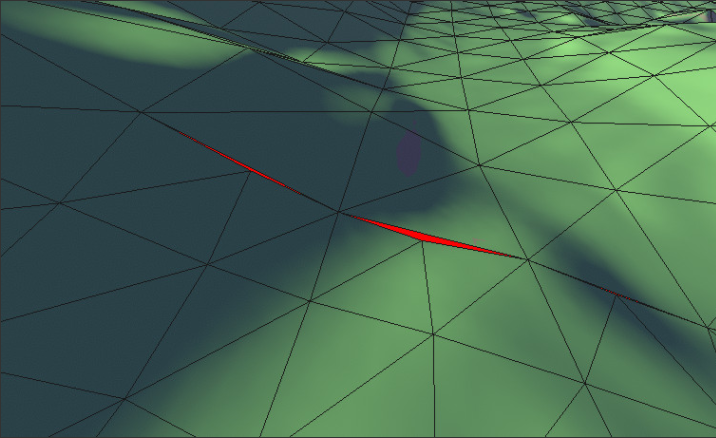
\includegraphics[width=6cm]{img/seams.png}
   \caption{Discontinuité http://mikejsavage.co.uk/blog/geometry-clipmaps.html}
   \label{fig:seams}
 \end{wrapfigure}
 
 \vspace{0.5cm}
 En effet la différence d'élévation entre chaque divisions peuvent provoquer une discontinuité provoquant ainsi une zone vide, 
 comme on peut le voir, par la zone rouge indiqué sur cette image. 
 
 
 \vspace{2.8cm}
 La méthode utilisé en général pour de palier à cette discontinuité est de rajouter des connexions entre les niveaux affectés. 
 Cette solution a de nombreux inconvéniant, en rajoutant des connexions de cette manière, lors du rendue et, lors du parcours du terrain ,ces connexions vont alors apparaitre brusquement perturbant ainsi la fluidité. À cela viennent s'ajouter la possibilité d'avoir des connexions multiple superposé et également un cout de rendue suplémentaire en terme de calcul et de mémoire.
 
 L'algorithme CDLOD va notamment ce différencier ici des autres algorithmes par ses "transitions fluides" entre les niveaux de détails par une méthode dites de "\textbf{morphing}" dont nous reparlerons après avoir expliqué l'algorithme plus en détails.
 
 Pour pouvoir correctement expliqué l'algorithme il est tout d'abord nécessaire d'introduire les notions de  \textbf{Heightmap} ainsi que de \textbf{Quadtree} quis sont des élements clef de l'algorithme.
 
  \section{Heightmap}
  
  Une Heightmap pour "Carte de hauteur" est une image permettant dans le cadre de rendue de terrain, de représenter le relief à l'aide de la nuance de gris. On peut ainsi interprété la nuance comme une hauteur par rapport à la surface. Le noir (une nuance nulle) représente la hauteur minimum et le blanc (une nuance maximal) réprésente la hauteur maximum. Des algorithmes permettent d'obtenir une carte de hauteur ressemblant à des \hl{terrains naturels}. Comme par exemple, l'algorithmes de bruit de perlin, bruit de simplex , déplacement du point médian...
  
  
  \section{Quadtree}
  
  

 \section{Chuncked LOD}
  
  L'algortihme \textbf{CDLOD}, est basé sur l'algorithme \textbf{CLOD} "Chuncked LOD" dévellopé par Thatcher Ulrich.
  Afin de mieux comprendre l'algorithme CDLOD il est donc nécessaire de présenter l'algorithme CLOD.
  
\begin{figure}[!h]
    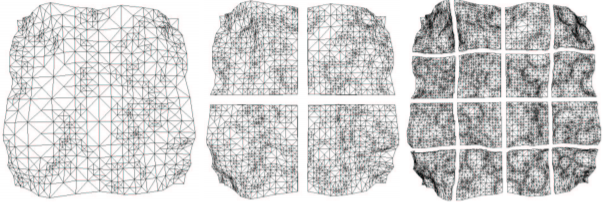
\includegraphics[width=12cm]{img/clod.png}
    \caption{CLOD http://tulrich.com/geekstuff/sig-notes.pdf}
    \label{fig:clod}
\end{figure}


  L'affichage des tronçons de terrain(chunck) est basé sur la distance de la caméra. Cela signigie que pour une certaine distance donné,
  les "chuncks" sont séléctionnés dans le Quadtree de façons à correspondre au terrain généré. Chaque tronçon 

  L'algorithme utilise un \textbf{Quadtree} pour stocker les différents "Level Of Detail". Lors de l'éxécution les LOD
  sont séléctionné dans le Quadtree et affiché. Dans le cas où des niveaux de détails différents sont voisins, des crevasses
  vont se former comme nous avont pue le voir précédemment. Pour corriger ce problème, Ulrich.T 


  

  	
  %-----------------------------------------------------------------%
  %   Architecture et explication détaillé de l'implémentation
  %-----------------------------------------------------------------%
  \chapter{Architecture du programme}
	
    
  
  \section{Système de rendu}
  \section{Génération du maillage}	% Explication de triangulator.
  % icosahèdre ?
  % triangulator ?
  % structure de données
	Il existe plusieurs manières de générer un maillage de planète, la méthode utilisé ici
	se base sur un icosahédron, une forme géométrique composée de douze sommets de base et 
	de vingt faces triangulaire. Chaque face étant un triangle équilateral de taille identique.
	La figure XX représente un icosahèdre.\\

	% Insert icosahedron image here	
	
	La génération du maillage et l'entierté de la partie LOD de l'algorithme se fait dans la classe Triangulator.
	L'arbre de données est implémenté avec la méthode des flux du CDLOD, c'est à dire que l'arbre n'est
	pas conservé en mémoire mais est regénérer à chaque itéation de la boucle. Les avantages de cette méthode seront 
	expliqué plus bas.
	
	Pour accélérer les temps d'accès mémoire, les distances avec les différents triangles sont conservées
	dans un tableau. \\

	Dans l'abre, chaque noeud possède trois positions correspondant aux trois points du triangle,
	ainsi que quatre pointeur vers ne niveaux suivant.
	D'autre information sont stocké comme un pointeur vers son parent, le niveau actuelle du
	noeud dans l'abre ou encore un tag correspondant au type du noeud.
	Le tag sous forme d'un enum permet de distinguer le noeud qui sont a l'interieur de l'abre de ceux
	qui ne le sont pas. Il permet aussi de renseigner si le noeud est une feuille.
		
	Pour chaque triangle, on commence par tester si le triangle est visible, c'est à dire si il est
	présent à l'interieur du cône de vision de la caméra. Si c'est la cas, on prend le centre de chaque
	arrete du triangle l'on recommence de manière récursive tans que une subdivision est nécessaire.
	C'est à dire tans que le noeud contenant le triangle n'est pas une feuille. Dans le cas contraire,
	
	\begin{figure}[!h]
    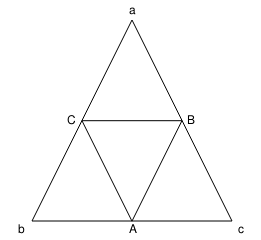
\includegraphics[width=12cm]{img/TriangleSplit.png}
    \caption{Division}
    \label{fig:TriangleSplit}
	\end{figure}
	
	La figure XX représente un diagramme de la fonction récursive. Lorsque l'on passe d'un niveau à un
	niveau inferieur dans l'arbre, le noeud courant pointer vers quatre fils, il est donc nécéssaire
	d'appeler récursivement quatre fois la fonction.
	
	On peut se rendre compte de la découpe du triangle en quatre plus petit dans la figure 
	\cite{TriangleSplit}.
	Les appels récursifs se font dans l'ordre aBC, AbC, ABc et enfin le triangle du milieux ABC.\\
	
	La fonction splitHeuristic permet en fonction de trois coordonnées représentant un triangle 
	et du niveau d'établir si ce triangle est dans le cône de vision ou non et de retourner le bon tag.
	Les méthodes permettant de déterminer si le cône de vision contient un triangle sont définies dans
	la classe Frustum.
	
  \section{Application du morphing}

  

  
  
  
  %-----------------------------------------------------------------%
  %   END
  %-----------------------------------------------------------------%
  
  \end{document}